\documentclass{article}
\usepackage[margin=1in]{geometry}
\usepackage{amsmath,amssymb}
\usepackage{parskip}
\usepackage{graphicx}
\usepackage{caption}
\usepackage{booktabs}
\DeclareMathOperator*{\argmin}{arg\,min}
\DeclareMathOperator*{\argmax}{arg\,max}

\title{CSE P 546 A - Homework 3}
\author{Thangakumar Dhanasekaran (2550520)}
\date{May-22-2026}

\begin{document}

\maketitle

\section*{A1}

\begin{enumerate}
  \item[(a)] \textbf{False.} Deep neural network loss functions are generally non-convex due to the composition of non-linear activations, so gradient descent can converge to a local minimum rather than the global optimum.

  \item[(b)] \textbf{False.} Initializing all weights to zero causes the symmetry problem: every neuron in a layer computes identical outputs and gradients, so they all update identically and the network never learns differentiated features. Random initialization breaks this symmetry.

  \item[(c)] \textbf{True.} Without non-linear activations, any composition of linear layers reduces to a single linear transformation, which can only learn linear decision boundaries. Non-linear activations are what allow the network to represent non-linear functions.

  \item[(d)] \textbf{False.} The backward pass traverses the same computation graph as the forward pass, so its time complexity is comparable (roughly $2\times$--$3\times$ the forward pass cost). It is not prohibitively larger.

  \item[(e)] \textbf{False.} Neural networks have high capacity but require large amounts of data and compute, and can be difficult to interpret. Simpler models (e.g., linear models, decision trees) are often preferable in low-data, resource-constrained, or interpretability-critical settings.
\end{enumerate}

\section*{A2}

\textbf{Claim.} For the feature map $\phi(x)$ whose $i$th component is
\[
  \phi_i(x) = \frac{1}{\sqrt{i!}}\,e^{-x^2/2}\,x^i, \quad i = 0, 1, 2, \ldots,
\]
the inner product satisfies $\phi(x)\cdot\phi(x') = e^{-(x-x')^2/2}$.

\begin{proof}
Compute the inner product directly by summing over all components $i \ge 0$:
\begin{align*}
  \phi(x)\cdot\phi(x')
  &= \sum_{i=0}^{\infty} \phi_i(x)\,\phi_i(x') \\
  &= \sum_{i=0}^{\infty}
       \left(\frac{1}{\sqrt{i!}}\,e^{-x^2/2}\,x^i\right)
       \left(\frac{1}{\sqrt{i!}}\,e^{-x'^2/2}\,x'^i\right) \\
  &= \sum_{i=0}^{\infty} \frac{1}{i!}\,e^{-(x^2+x'^2)/2}\,(xx')^i \\
  &= e^{-(x^2+x'^2)/2} \sum_{i=0}^{\infty} \frac{(xx')^i}{i!}.
\end{align*}

By the Taylor expansion $e^z = \displaystyle\sum_{i=0}^{\infty}\frac{z^i}{i!}$
applied with $z = xx'$, the sum equals $e^{xx'}$.  Therefore,
\begin{align*}
  \phi(x)\cdot\phi(x')
  &= e^{-(x^2+x'^2)/2}\cdot e^{xx'} \\
  &= e^{-(x^2 - 2xx' + x'^2)/2} \\
  &= e^{-(x-x')^2/2}.
\end{align*}

Hence $K(x,x') = e^{-(x-x')^2/2}$ is a valid kernel for $\phi$.
\end{proof}

\section*{A3}

\subsection*{Part a — Optimal hyperparameters (LOO cross-validation on $n=30$)}

\begin{center}
\begin{tabular}{lll}
\toprule
Kernel & $\lambda$ & Kernel parameter \\
\midrule
RBF      & $2.21 \times 10^{-3}$ & $\gamma = 10.54$ (median heuristic) \\
Polynomial & $3.73 \times 10^{-5}$ & $d = 16$ \\
\bottomrule
\end{tabular}
\end{center}

\subsection*{Part b — Predictions on a fine grid}

\begin{figure}[h]
  \centering
  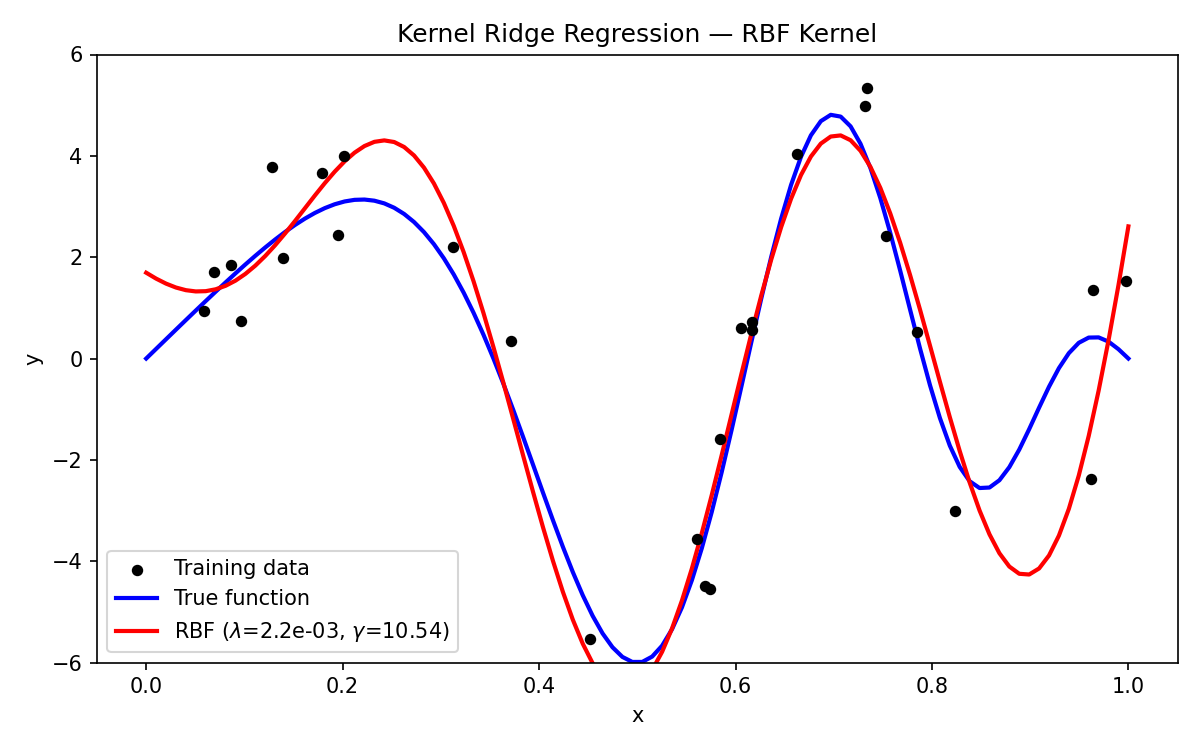
\includegraphics[width=0.85\textwidth]{a3_rbf_prediction.png}
  \caption{Kernel ridge regression with RBF kernel
    ($\lambda = 2.21\times10^{-3}$, $\gamma = 10.54$) trained on $n=30$ points.
    The red curve is the learned predictor; blue is the true function
    $f(x) = 6\sin(\pi x)\cos(4\pi x^2)$.}
\end{figure}

\begin{figure}[h]
  \centering
  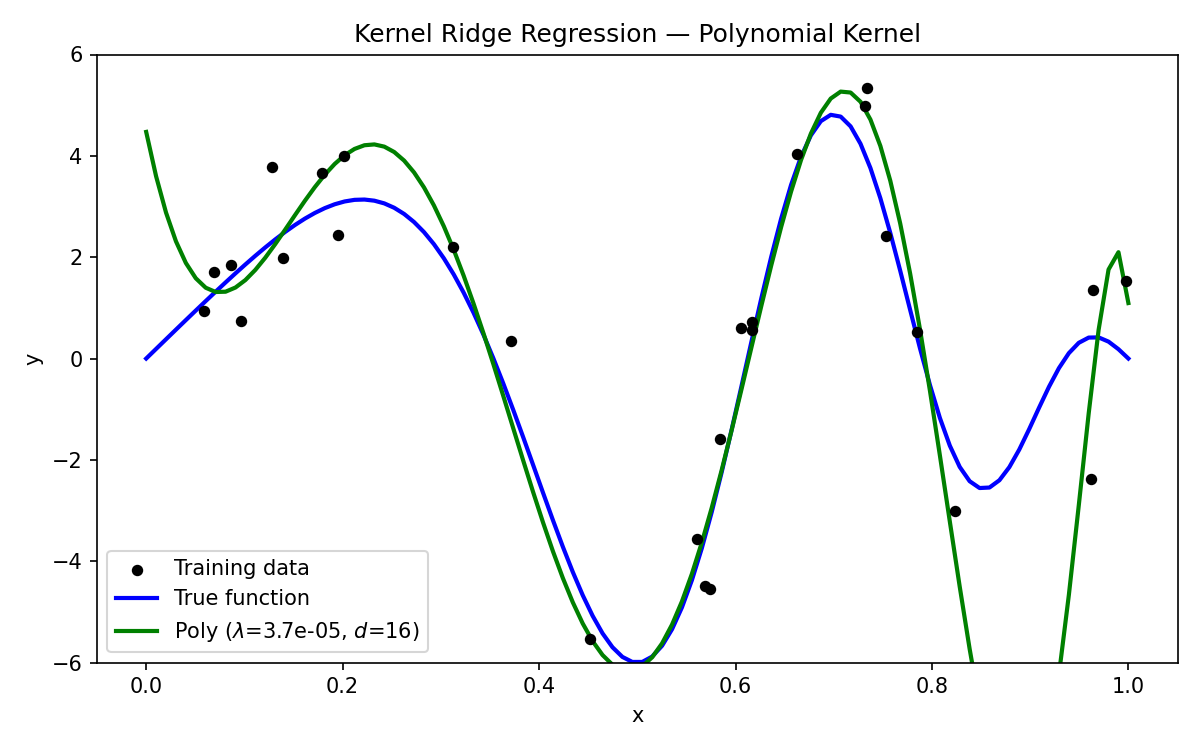
\includegraphics[width=0.85\textwidth]{a3_poly_prediction.png}
  \caption{Kernel ridge regression with polynomial kernel
    ($\lambda = 3.73\times10^{-5}$, $d = 16$) trained on $n=30$ points.
    The green curve is the learned predictor; blue is the true function.}
\end{figure}

\clearpage

% ─────────────────────────────────────────────────────────────────────────────
\section*{A4}

\subsection*{Part a — Problem Setup}

We train six neural-network architectures on the XOR binary-classification
dataset using two different loss functions: Mean-Squared Error (MSE) and
Cross-Entropy (CE).
Both experiments share the same six architectures (in this order):
\begin{enumerate}
  \item \textbf{Linear} — single linear layer (input $\to$ output, no hidden layer).
  \item \textbf{1-hidden-Sigmoid} — one hidden layer of size 2 with sigmoid activation.
  \item \textbf{1-hidden-ReLU} — one hidden layer of size 2 with ReLU activation.
  \item \textbf{2-hidden-Sigmoid-ReLU} — two hidden layers of size 2 with Sigmoid then ReLU activations.
  \item \textbf{2-hidden-ReLU-Sigmoid} — two hidden layers of size 2 with ReLU then Sigmoid activations.
  \item \textbf{2-hidden-ReLU-ReLU} — two hidden layers of size 2 with ReLU activations on both.
\end{enumerate}
CE models additionally end with a Softmax layer (required by the CE loss
implementation), while MSE models output raw logits matched to one-hot targets.
All models are trained with SGD ($\eta = 0.1$, batch size 32) for 200 epochs.
The best model is selected as the one achieving the lowest validation loss at
\emph{any} point during training.

\subsection*{Part b — Training and Validation Loss Curves}

\begin{figure}[h]
  \centering
  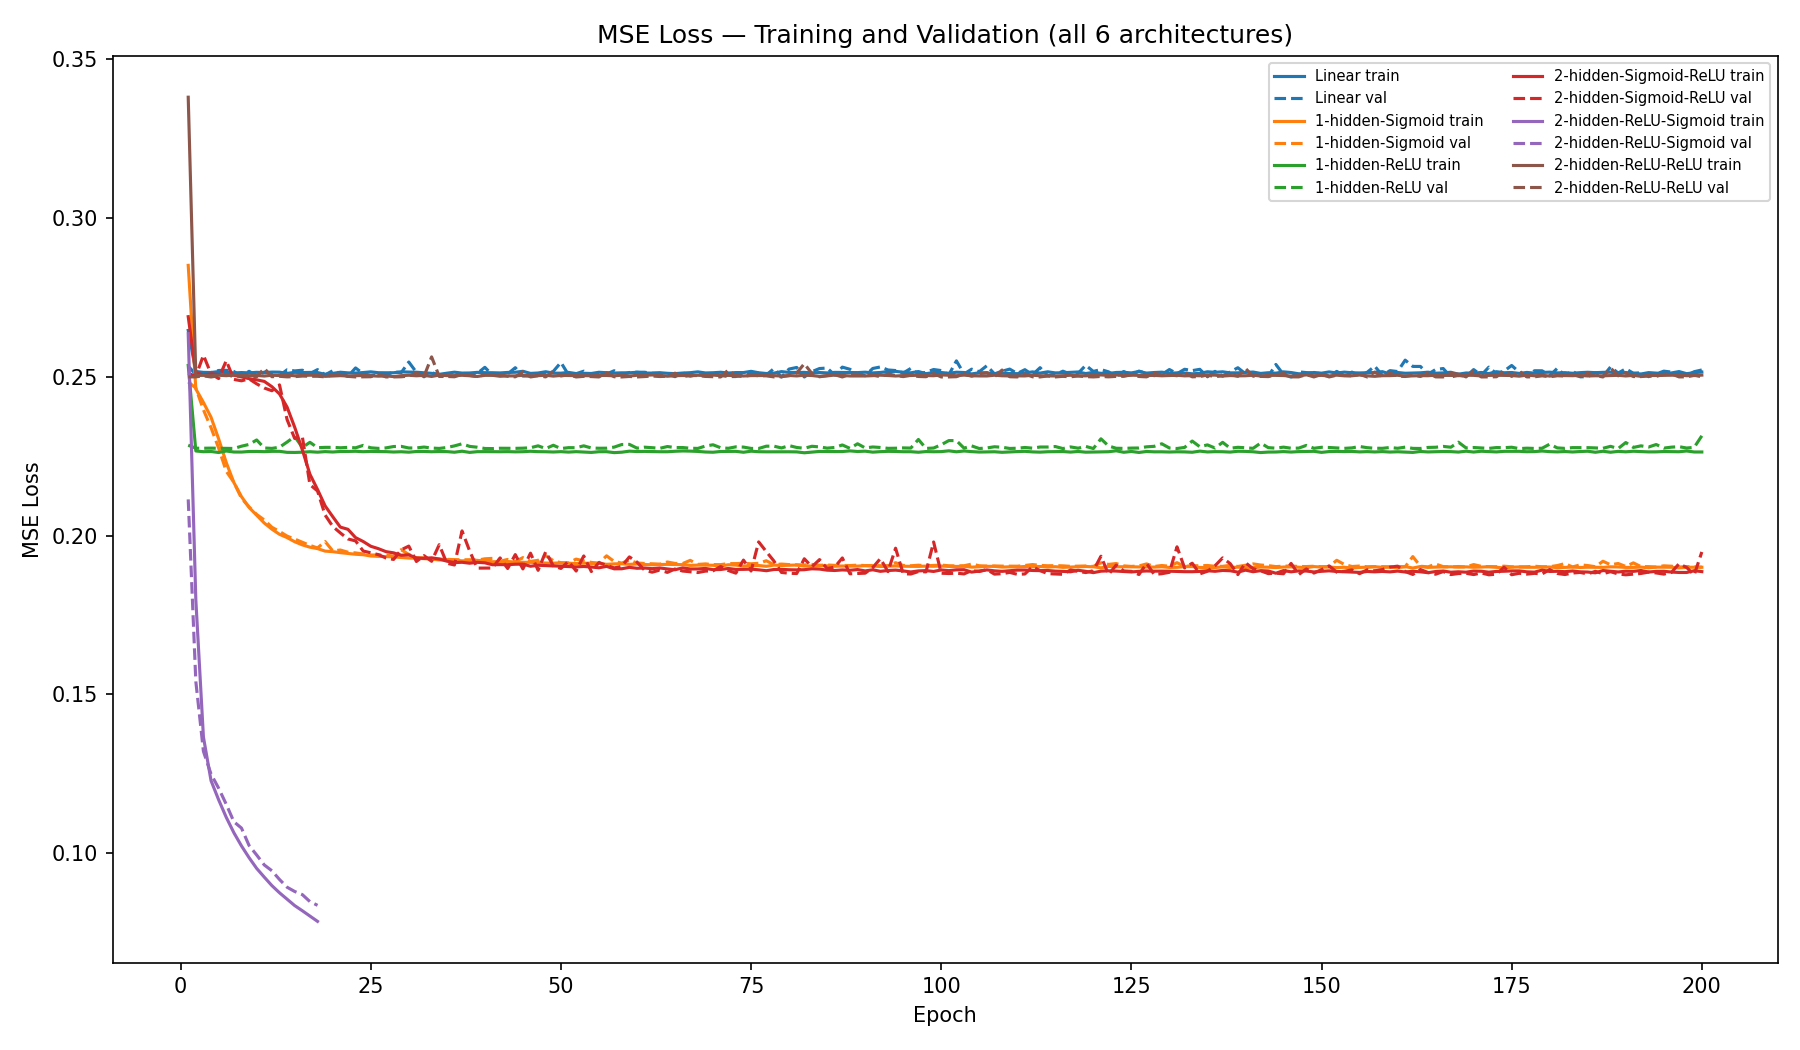
\includegraphics[width=0.95\textwidth]{a4_mse_loss.png}
  \caption{MSE loss (train = solid, validation = dashed) for all six
    architectures over 200 epochs (12 lines total).}
\end{figure}

\begin{figure}[h]
  \centering
  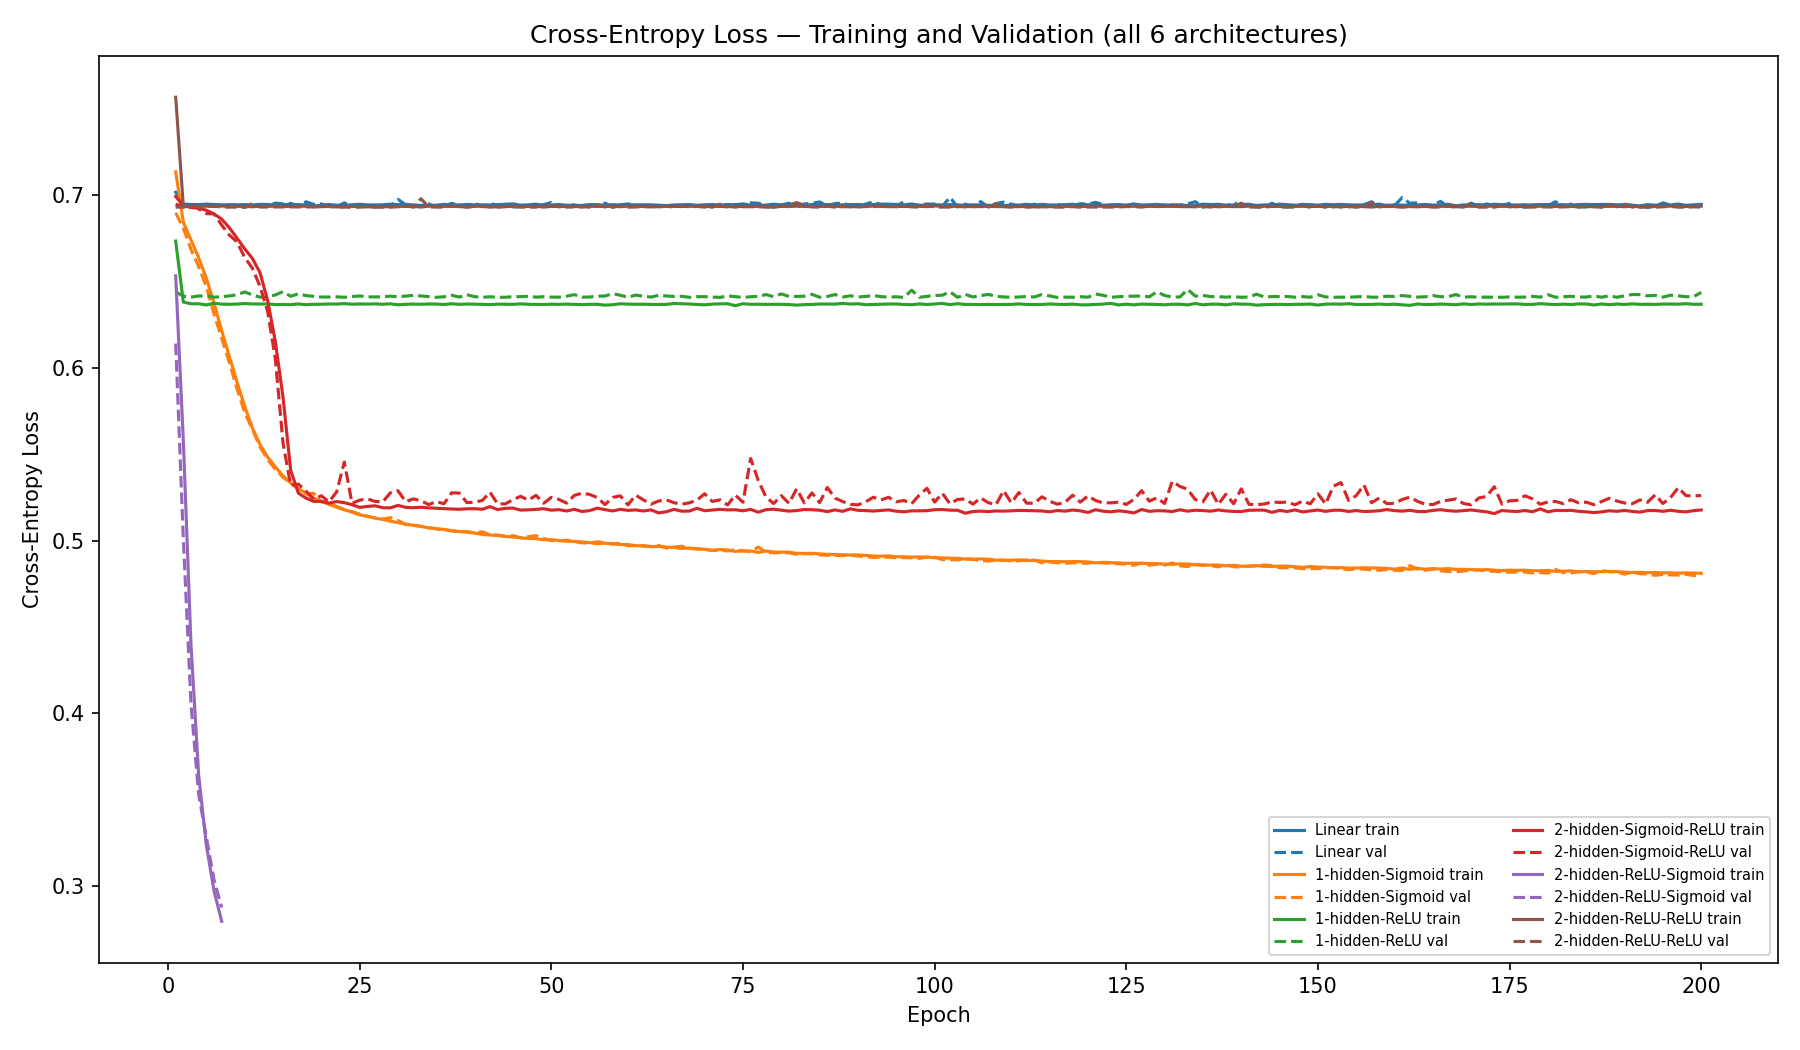
\includegraphics[width=0.95\textwidth]{a4_ce_loss.png}
  \caption{Cross-Entropy loss (train = solid, validation = dashed) for all six
    architectures over 200 epochs (12 lines total).}
\end{figure}

\subsection*{Part c — Best Architectures and Test-Set Predictions}

\textbf{MSE best model:} \texttt{2-hidden-ReLU-Sigmoid} — two hidden layers of size 2
with ReLU activation after the first hidden layer and Sigmoid after the second.
Best validation MSE $= 0.0836$. \textbf{Test accuracy: 91.02\%}.

\textbf{CE best model:} \texttt{2-hidden-ReLU-Sigmoid} — same architecture as above.
Best validation cross-entropy $= 0.2877$. \textbf{Test accuracy: 91.86\%}.

Both loss functions selected the same best architecture: two hidden layers (size 2 each)
with ReLU then Sigmoid activations, suggesting that this combination of activations
provides the most useful non-linearity for the XOR decision boundary at this
network width.

\begin{figure}[h]
  \centering
  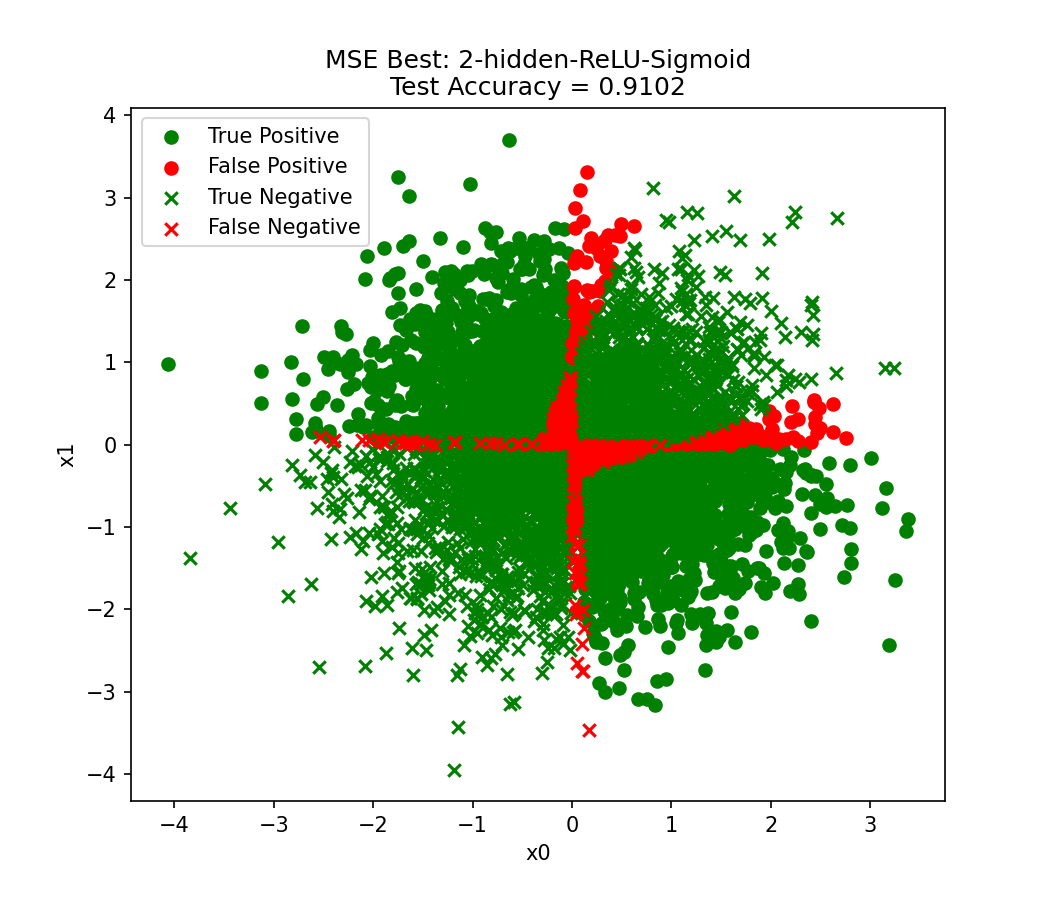
\includegraphics[width=0.7\textwidth]{a4_mse_predictions.png}
  \caption{Test-set predictions of the best MSE model on the XOR dataset.
    Points are coloured by TP/FP/TN/FN classification.}
\end{figure}

\begin{figure}[h]
  \centering
  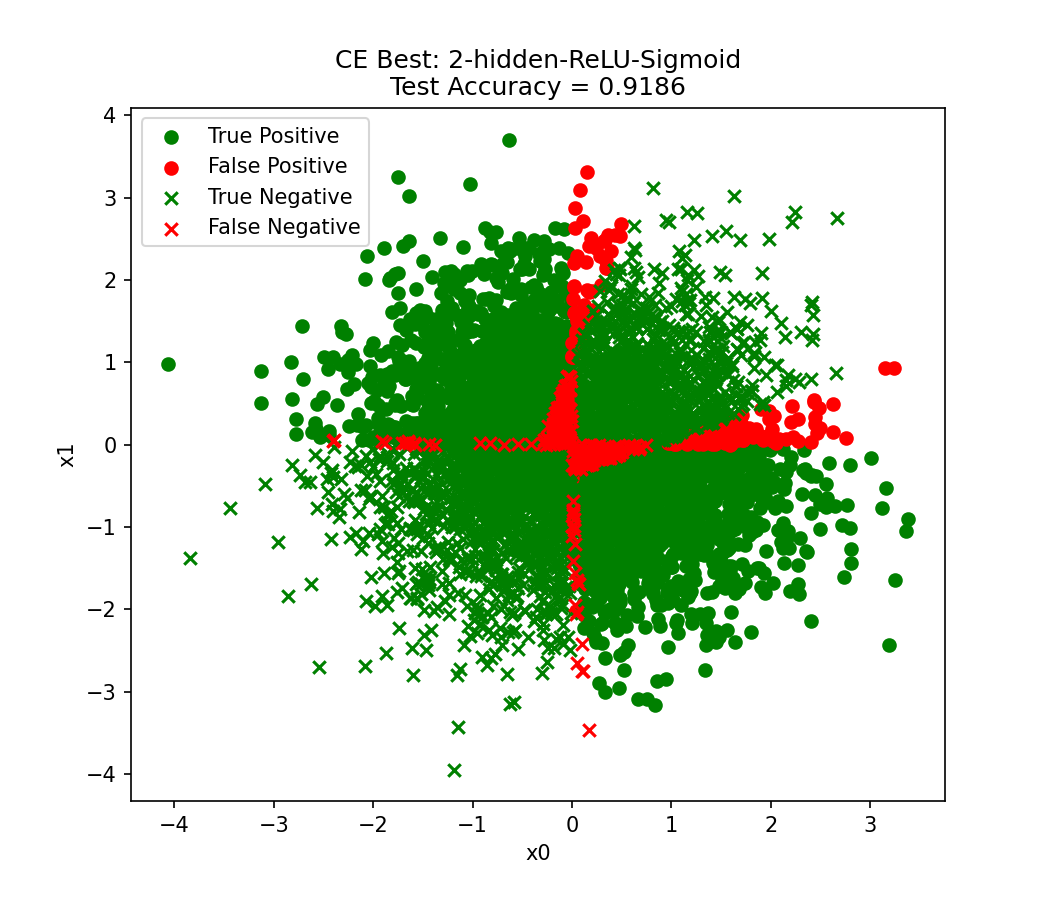
\includegraphics[width=0.7\textwidth]{a4_ce_predictions.png}
  \caption{Test-set predictions of the best CE model on the XOR dataset.
    Points are coloured by TP/FP/TN/FN classification.}
\end{figure}

\clearpage

% ─────────────────────────────────────────────────────────────────────────────
\section*{A5}

\subsection*{Parts a--b — Training Loss and Test Performance}

We implement two feed-forward networks from scratch using only
\texttt{torch.nn.functional.relu} and \texttt{torch.nn.functional.cross\_entropy}
(no other \texttt{torch.nn} components):
\begin{itemize}
  \item \textbf{F1} — one hidden layer of size $h=64$:
    $\mathbf{x} \xrightarrow{W_0,b_0} \text{ReLU} \xrightarrow{W_1,b_1} \text{logits}$.
  \item \textbf{F2} — two hidden layers of sizes $h_0=32,\,h_1=32$:
    $\mathbf{x} \xrightarrow{W_0,b_0} \text{ReLU} \xrightarrow{W_1,b_1} \text{ReLU} \xrightarrow{W_2,b_2} \text{logits}$.
\end{itemize}
Both networks use Uniform$(-1/\sqrt{d_\text{in}},\,1/\sqrt{d_\text{in}})$
weight initialisation and are trained with Adam ($\eta=10^{-3}$, batch size 256)
until training accuracy reaches 99\%.

\begin{figure}[h]
  \centering
  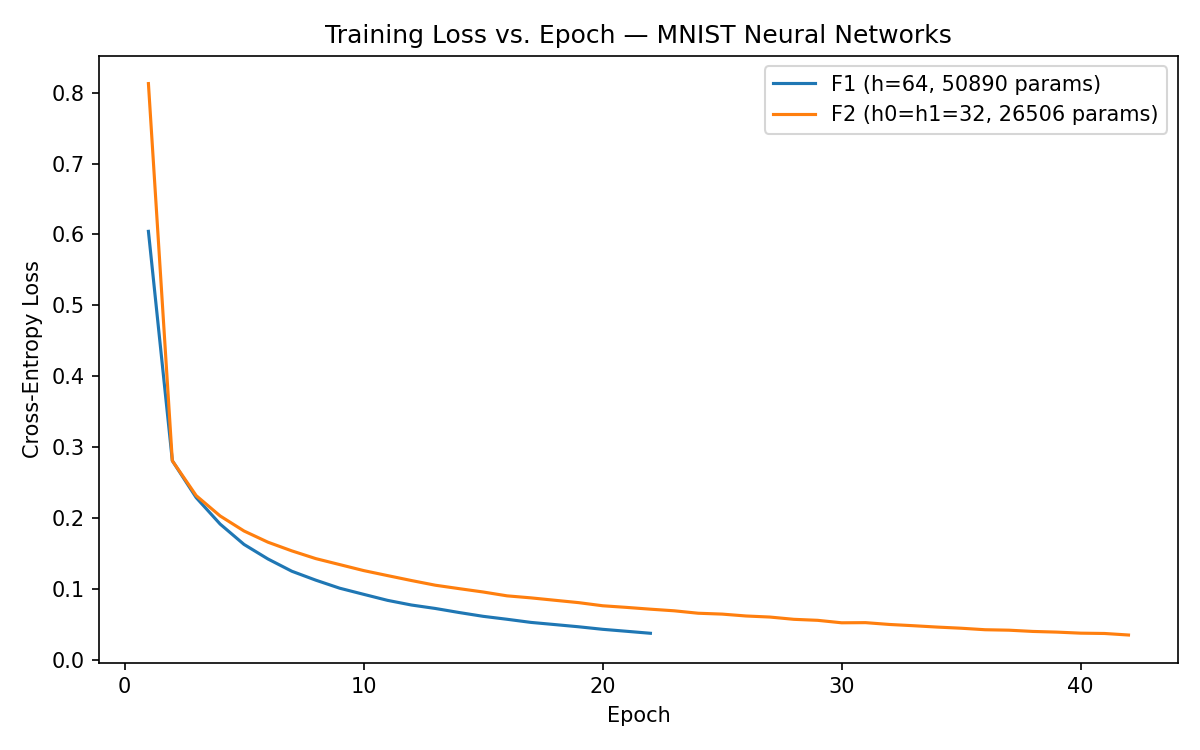
\includegraphics[width=0.85\textwidth]{a5_training_loss.png}
  \caption{Cross-entropy training loss per epoch for F1 and F2 on MNIST.}
\end{figure}

\begin{center}
\begin{tabular}{lll}
\toprule
Model & Test Accuracy & Test CE Loss \\
\midrule
F1 ($h=64$)       & 97.50\% & 0.0834 \\
F2 ($h_0=h_1=32$) & 96.85\% & 0.1187 \\
\bottomrule
\end{tabular}
\end{center}

\subsection*{Part c — Parameter Counts and Comparison}

\begin{center}
\begin{tabular}{lll}
\toprule
Model & Architecture & Parameters \\
\midrule
F1 & $784\!\to\!64\!\to\!10$ & $784\times64+64+64\times10+10 = 50{,}890$ \\
F2 & $784\!\to\!32\!\to\!32\!\to\!10$ & $784\times32+32+32\times32+32+32\times10+10 = 26{,}506$ \\
\bottomrule
\end{tabular}
\end{center}

F1 uses roughly twice as many parameters as F2 and achieves slightly higher test
accuracy (97.50\% vs.\ 96.85\%), suggesting that for MNIST the extra width of a
single wider hidden layer is more beneficial than adding depth with smaller hidden
layers at this parameter scale.

\clearpage

% ─────────────────────────────────────────────────────────────────────────────
\section*{A6}

\subsection*{Part a — Cross-Entropy Loss and Gradient}

For a single example $(x_i, y_i)$ the cross-entropy loss is
\[
  L_i(W) = -\log p(y_i \mid x_i;\,W)
          = -W_{y_i}^\top x_i + \log\!\sum_{\ell=1}^{k} \exp\!\bigl(W_\ell^\top x_i\bigr).
\]

\textbf{Gradient derivation.}
We compute $\nabla_{W_j} L_i(W)$ for each column $W_j \in \mathbb{R}^d$ of $W$.

\textit{Term 1:} $\dfrac{\partial}{\partial W_j}\bigl(-W_{y_i}^\top x_i\bigr) = -\mathbf{1}[j = y_i]\,x_i.$

\textit{Term 2:} $\dfrac{\partial}{\partial W_j}\log\!\displaystyle\sum_\ell \exp(W_\ell^\top x_i)
  = \dfrac{\exp(W_j^\top x_i)}{\displaystyle\sum_\ell \exp(W_\ell^\top x_i)}\,x_i
  = p(j \mid x_i;\,W)\,x_i.$

Adding both terms:
\[
  \boxed{\nabla_{W_j} L_i(W) = \bigl(p(j \mid x_i;\,W) - \mathbf{1}[j = y_i]\bigr)\,x_i.}
\]

\subsection*{Part b — Training Results}

We train a multinomial logistic regression model on MNIST ($d=784$, $k=10$) using
SGD ($\eta=0.1$, batch size 256, 50 epochs) with two loss functions:
\begin{itemize}
  \item $J\text{-loss}$ — joint negative log-likelihood (sum over all examples).
  \item $L\text{-loss}$ — standard average cross-entropy (mean over examples).
\end{itemize}

\begin{center}
\begin{tabular}{lll}
\toprule
Loss & Train Accuracy & Test Accuracy \\
\midrule
$J$-loss & 91.72\% & 90.66\% \\
$L$-loss & 92.45\% & 92.24\% \\
\bottomrule
\end{tabular}
\end{center}

$L$-loss converges more smoothly (the gradient scale is fixed regardless of batch size),
while $J$-loss is noisier because summing over the full batch amplifies mini-batch
size variation in the gradient magnitude.

\begin{figure}[h]
  \centering
  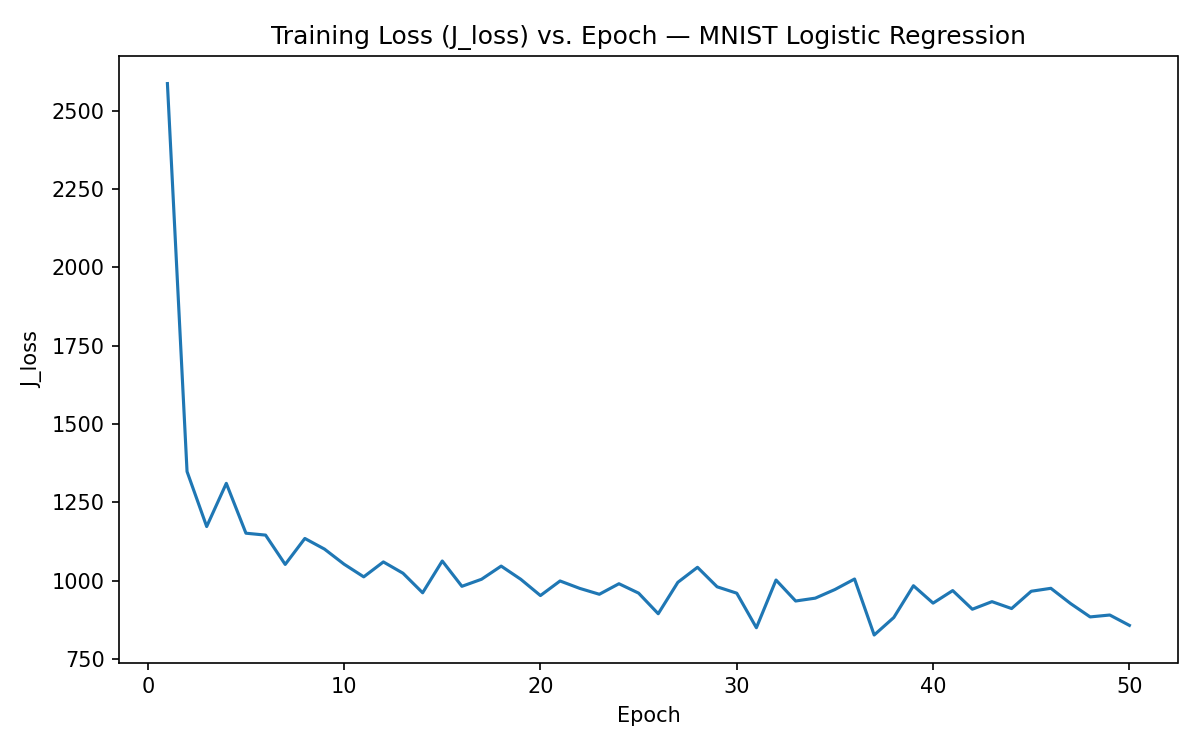
\includegraphics[width=0.85\textwidth]{a6_j_loss.png}
  \caption{Training loss ($J$-loss, sum of NLL) vs.\ epoch for multinomial
    logistic regression on MNIST.}
\end{figure}

\begin{figure}[h]
  \centering
  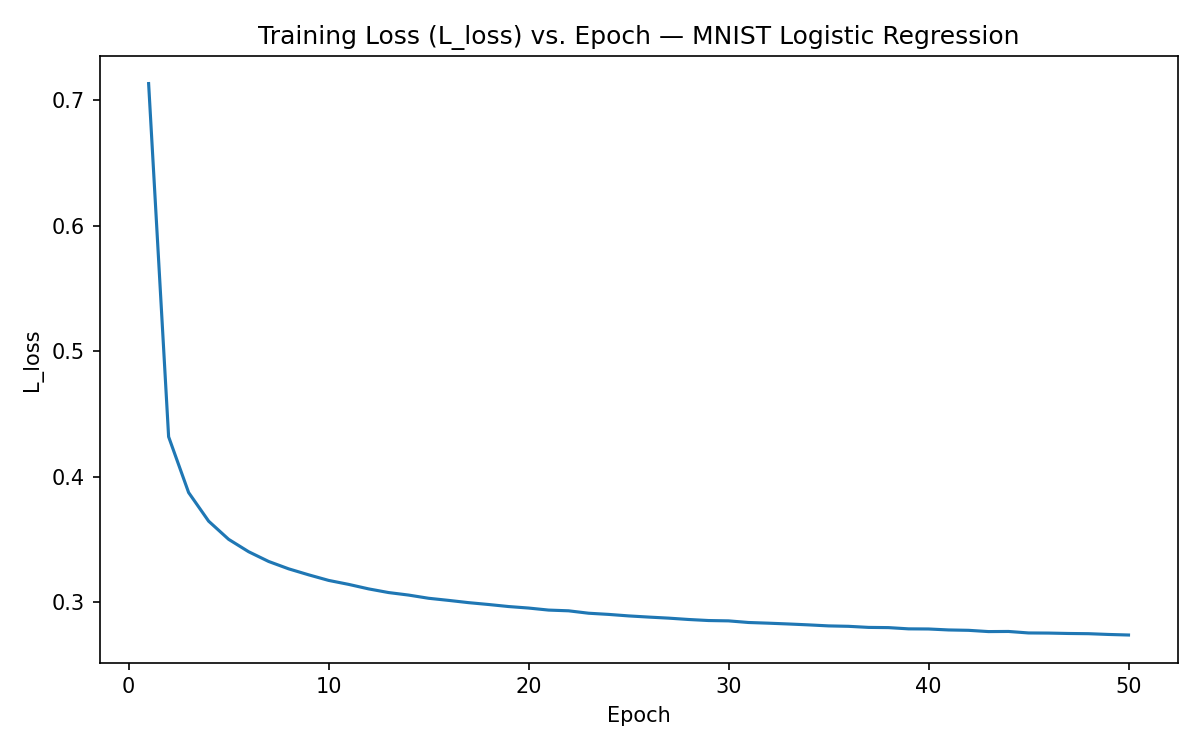
\includegraphics[width=0.85\textwidth]{a6_l_loss.png}
  \caption{Training loss ($L$-loss, mean NLL / standard cross-entropy) vs.\ epoch
    for multinomial logistic regression on MNIST.}
\end{figure}

\clearpage

\end{document}